\documentclass{article}  % Define la clase del documento.

% Paquetes de idioma y codificación
\usepackage[utf8]{inputenc}
\usepackage[T1]{fontenc}
\usepackage[spanish]{babel}  % Ajusta el idioma del documento a español.
\usepackage{tabularx}  % Permite la creación de tablas con ancho ajustable.

% Paquete de geometría para configurar márgenes y tamaño de papel
\usepackage[letterpaper, margin=3cm]{geometry}
\usepackage{caption}

% Paquetes de tipografía
\usepackage{mathptmx}    % Usa Times New Roman como fuente.
\usepackage{microtype}   % Mejora la justificación del texto.
\usepackage{multicol}
% Paquetes para manejo de colores y gráficos
\usepackage{xcolor}      % Define y utiliza colores.
\usepackage{graphicx}    % Permite la inserción de imágenes.
\usepackage{tikz}        % Creación de gráficos vectoriales.

% Configuración de enlaces y referencias cruzadas
\usepackage{hyperref}
\hypersetup{
    colorlinks   = true,
    linkcolor    = darkblue,
    citecolor    = black,
    filecolor    = blue,
    urlcolor     = blue
}

\usepackage{media9} % Permite la inserción de multimedia.

% Paquetes para la mejora visual de tablas y figuras
\usepackage{booktabs}    % Para tablas de alta calidad.
\usepackage{float}       % Controla la posición de figuras y tablas.

% Paquete para la personalización de códigos fuente
\usepackage{listings}
\lstset{
    literate=
    {á}{{\'a}}1 {é}{{\'e}}1 {í}{{\'i}}1 {ó}{{\'o}}1 {ú}{{\'u}}1
    {Á}{{\'A}}1 {É}{{\'E}}1 {Í}{{\'I}}1 {Ó}{{\'O}}1 {Ú}{{\'U}}1
    {ñ}{{\~n}}1 {Ñ}{{\~N}}1 {ü}{{\"u}}1 {Ü}{{\"U}}1,
    backgroundcolor=\color{backcolour},
    commentstyle=\color{codegreen},
    keywordstyle=\color{codepurple},
    numberstyle=\tiny\color{codegray},
    stringstyle=\color{red},
    basicstyle=\ttfamily\small,
    breakatwhitespace=false,
    breaklines=true,
    captionpos=b,
    keepspaces=true,
    numbers=left,
    numbersep=5pt,
    showspaces=false,
    showstringspaces=false,
    showtabs=false,
    tabsize=2,
    language=TeX,
    morecomment=[l]\#,
    frame=single,
    rulecolor=\color{black}
}

% Definición de colores al estilo Visual Studio Code
\definecolor{darkblue}{rgb}{0.0, 0.0, 0.55}  % Enlaces
\definecolor{codegreen}{rgb}{0.25, 0.49, 0.48}  % Comentarios
\definecolor{codegray}{rgb}{0.5, 0.5, 0.5}  % Números y anotaciones
\definecolor{codepurple}{rgb}{0.58, 0, 0.82}  % Palabras clave
\definecolor{backcolour}{rgb}{0.95, 0.95, 0.92}  % Fondo de código

% Configuraciones de párrafo y matemáticas
\usepackage{amsmath}
\usepackage{parskip}    % Espaciado entre párrafos.
\usepackage{ragged2e}   % Justificación mejorada.

% Configuración de secciones y encabezados
\usepackage{titlesec}
\titleclass{\part}{top}
\titleformat{\part}[display]
  {\normalfont\huge\bfseries\centering}{\thepart}{40pt}{\Huge}
\titlespacing*{\part}{0pt}{-60pt}{10pt}
\titleformat{\part}
  {\normalfont\huge\bfseries}{}{0pt}{}
\titleformat{\part}[display]
  {\normalfont\huge\bfseries}{}{0pt}{}
  [\thispagestyle{fancy}]

% Encabezado y pie de página
\usepackage{fancyhdr}
\pagestyle{fancy}
\fancyhf{}
\fancyhead[L]{\raisebox{0.20cm}{\textbf{EPI}}}
\fancyhead[R]{\raisebox{0.1cm}{
\includegraphics[width=0.25\linewidth]{LOGO_UNIVERSIDAD.jpg}}}
\fancyhead[C]{\rule{\textwidth}{0.6pt}}
\fancyfoot[C]{\rule{\textwidth}{0.6pt}}
\fancyfoot[R]{\raisebox{-1.5\baselineskip}{\thepage}}
\renewcommand{\headrulewidth}{0pt}
\renewcommand{\footrulewidth}{0pt}

% Geometría avanzada
\geometry{
  top=3.5cm,
  bottom=2.5cm,
  headheight=2.5cm
}

% Bibliografía
\usepackage{natbib}
\bibliographystyle{unsrtnat}

\begin{document}

%---------------------------------------- PORTADA ----------------------------------------
\begin{titlepage}
\newcommand{\HRule}{\rule{\linewidth}{0.5mm}} 
\center

\includegraphics[width=10cm]{LOGO_UNIVERSIDAD.jpg}\\
\vspace{3cm}
\HRule \\[0.4cm]
{ \huge \bfseries Prueba 2}\\[0.4cm]
{ \huge \bfseries EPI}\\[0.4cm]
\HRule \\[1.5cm]
\vspace{4.5cm}
\begin{flushright}
    \vspace{0.8cm}
    \textbf{Alumnos:} \\
    Bernardo Caprile\\
    Lukas Wolff Casanova\\
\end{flushright}
\vspace{1cm}
{\large \textbf{\today}}\\[2cm]
\end{titlepage}



\newpage
\setcounter{page}{1}

%---------------------------------------- CONTENIDO ----------------------------------------
\section{Target Value Design (TVD)}

Metodo que se ideo con el objetivo de conducir el diseño y construccion de un proyecto
hacia el \textbf{logro de los objetivos}

Se busca hacer una adatacion del \textbf{target costing} 

Las diferencias entre el diseño convencional y el TVD son:

\begin{table}[h!]
\centering
\begin{tabular}{|p{6.5cm}|p{6.5cm}|}
\hline
\textbf{TVD} & \textbf{Práctica tradicional} \\
\hline
Ciclo de diseño – estimación – rediseño & Ciclo de diseño – estimación – retrabajo \\
\hline
Se elabora primero un estimado y entonces el diseño es realizado alineándose con el estimado. & El diseño multidisciplinario es dibujado y entonces se hace el estimado en función de él. \\
\hline
El diseño se basa solo en lo que se puede construir. & Es necesaria una evaluación del diseño respecto a constructabilidad. \\
\hline
Todos los diseñadores se involucran desde el diseño inicial. & El arquitecto diseña, entonces otros involucrados basan su trabajo en el proyecto de arquitecto. \\
\hline
El costo objetivo nunca debe ser excedido. & El costo del proyecto excede lo que el cliente puede pagar por él. \\
\hline
\end{tabular}
\caption{Comparación entre TVD y práctica tradicional}
\end{table}

Ahora, para poder llevar a cabo el TVD, se deben cumplir los siguientes aspectos:

\begin{itemize}
    \item Integracion Temprana
    \item Compartir Riesgos y Recomensas
    \item Tener Objetivos Alineados
    \item Diseño Concurrente, compartir el conocimiento sobre costos y experiencias.
\end{itemize}

\begin{figure}[H]
\centering
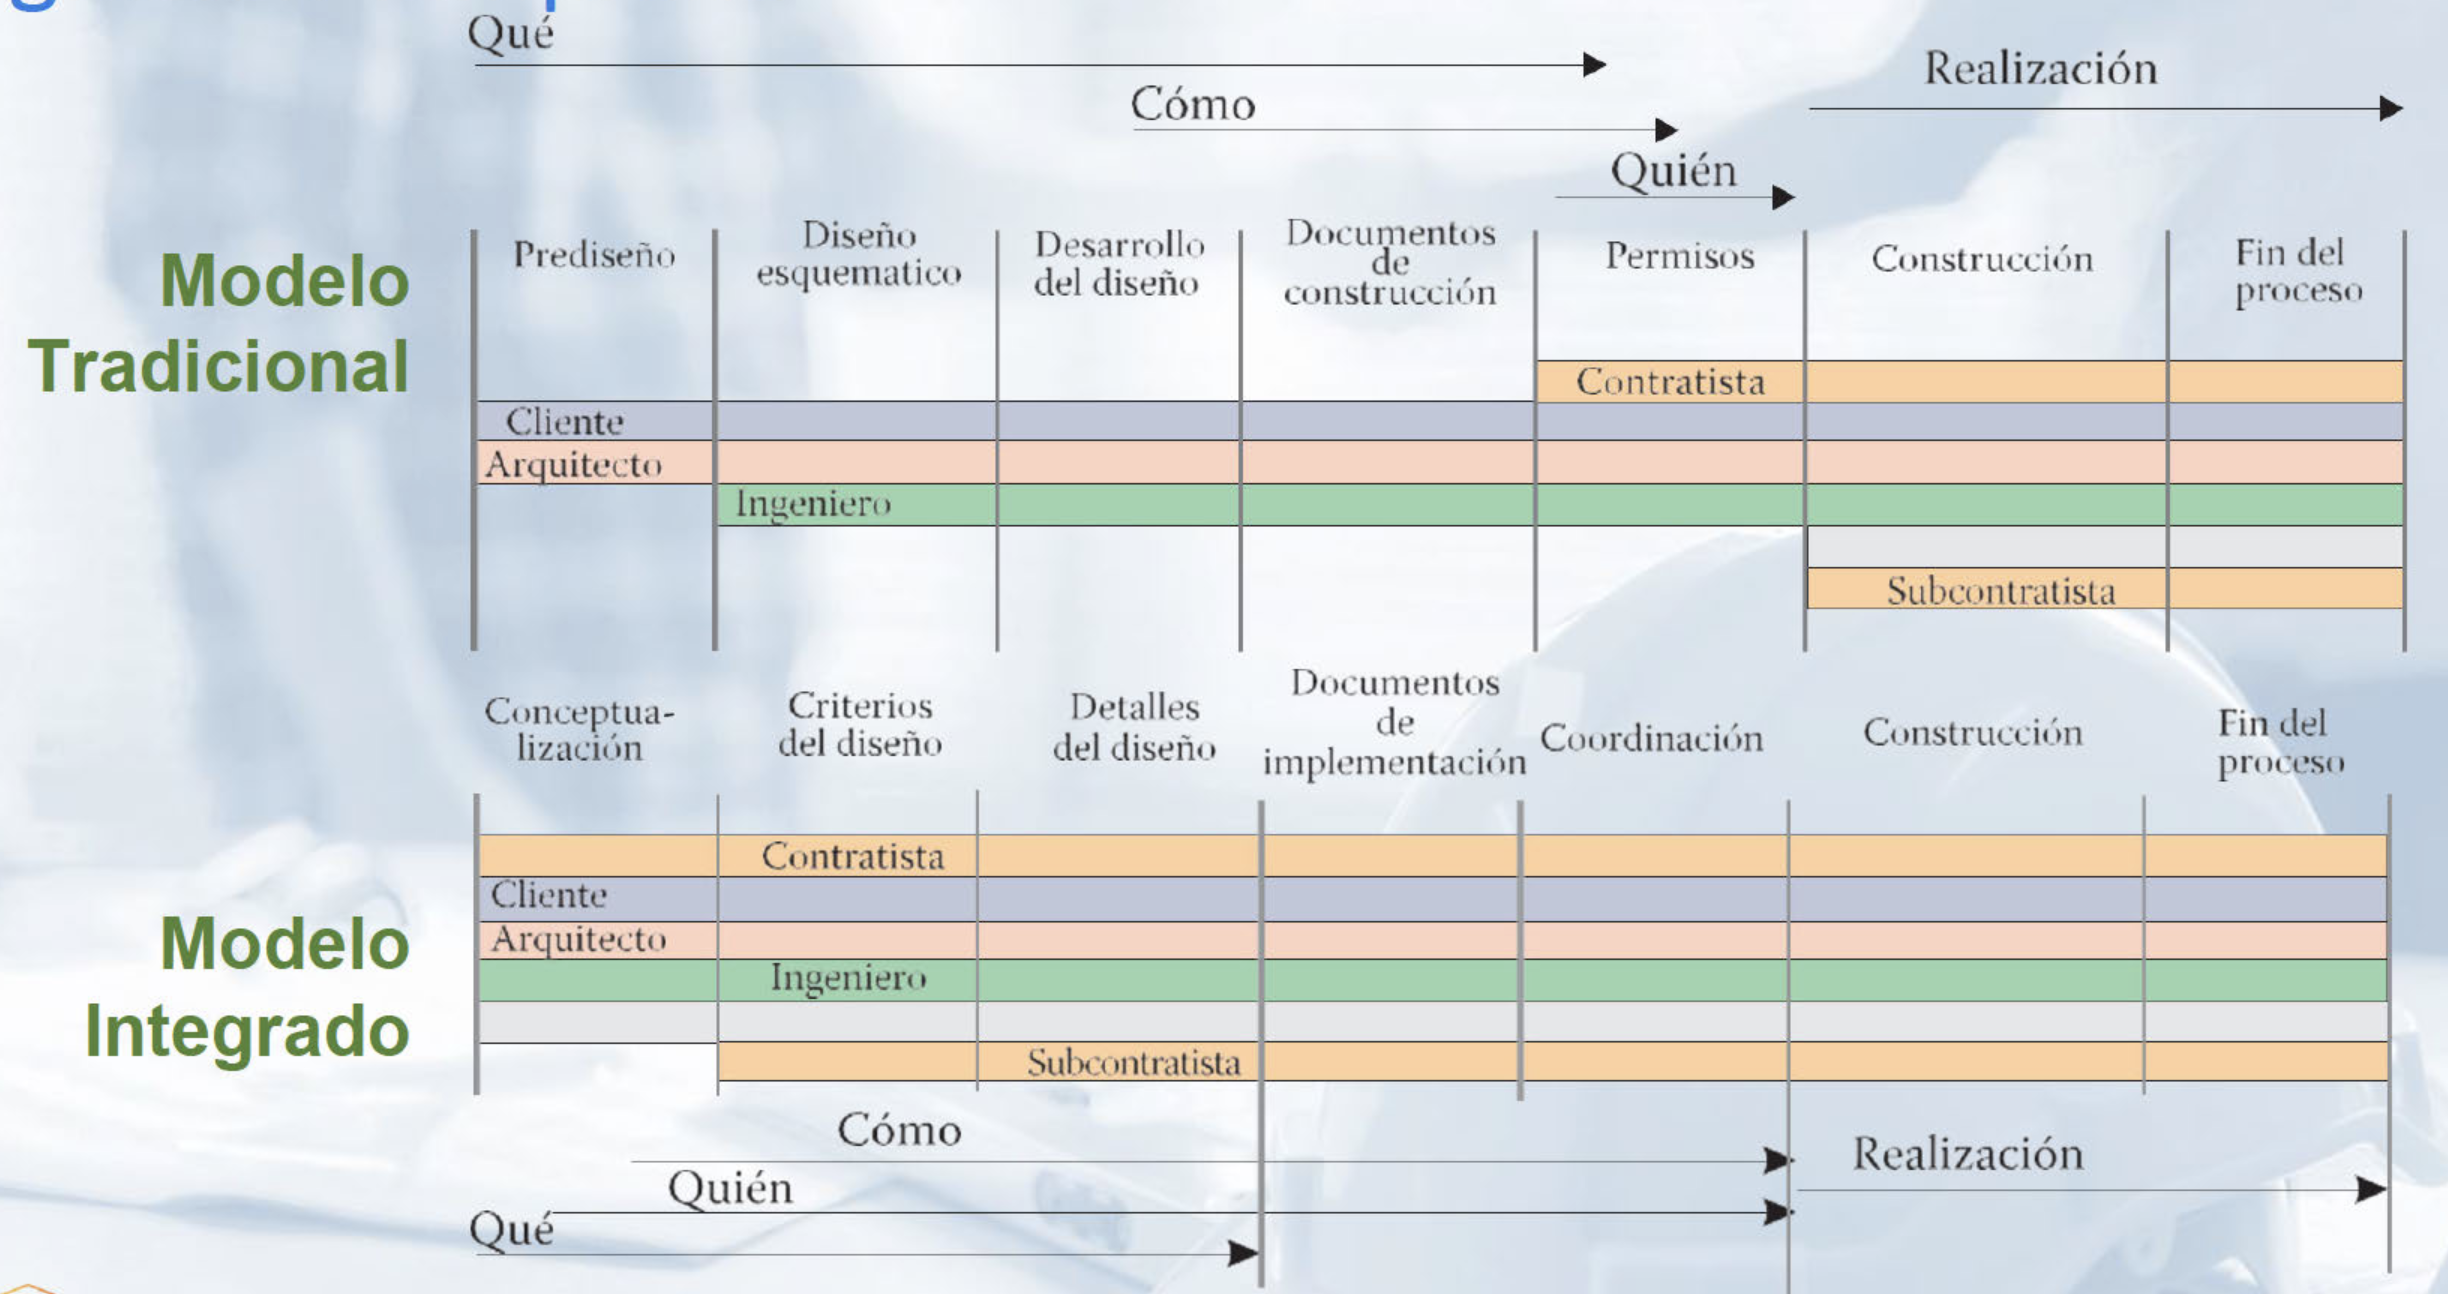
\includegraphics[width=0.8\textwidth]{IMAGENES/TVD.png}
\caption{Proceso de TVD}
\label{fig:tvd}
\end{figure}

Los pasos a ejecutar son:

\begin{itemize}
    \item Definir el costo objetivo para el proyecto
    \item Trabajar estructuradamente
    \item Colaboracion
    \item Set-Based Design
    \item Collocation
\end{itemize}

Ahora bien, algunas buenas practicas a seguir dentro de TVD son:

\begin{itemize}
    \item Comprometerse con el cliente para \textbf{establecer valor objetivo}
    \item Guiar los esfuerzos de diseño hacia el \textbf{aprendizaje y la innovación}
    \item \textbf{Diseñar} en relación con el \textbf{presupuesto y el valor objetivo} del cliente
    \item Planear \textbf{colaborativamente}
    \item Diseñar simultáneamente el \textbf{producto y el proceso}
    \item Diseñar y planear con base en el \textbf{cliente} que utilizará el producto
    \item Trabajar en \textbf{pequeños grupos} multidisciplinarios
    \item Trabajar en un “Big room”. \textbf{Co-location}
    \item Realizar \textbf{retrospectivas} a lo largo del proceso
\end{itemize}

\subsection{Como trabajar en TVD}

De esta forma, se ontiene lo siguiente:


\noindent En lugar de diseñar aisladamente y posteriormente reunirse para revisiones y decisiones de grupo, \textbf{colaboración} 
\[
\Rightarrow \text{Trabajar en equipo para definir los inconvenientes y decisiones y luego diseñar conforme a esas decisiones}
\]

\noindent En lugar de evaluar la constructabilidad del diseño, \textbf{estructura de trabajo}
\[
\Rightarrow \text{Diseñar lo que es construible}
\]

\noindent En lugar de trabajar solos en cuartos separados, \textbf{co-locación}
\[
\Rightarrow \text{Trabajar en parejas o en grupos más grandes, cara a cara}
\]

\noindent En lugar de estimar con base en un diseño detallado, \textbf{costo objetivo}
\[
\Rightarrow \text{Diseñar con base en un estimado detallado}
\]

\noindent En lugar de tomar decisiones que reduzcan las posibilidades para proceder con el diseño, \textbf{Set Based Design}
\[
\Rightarrow \text{Mantener conjuntos de decisiones abiertos a lo largo del proceso de diseño}
\]

\subsection{Beneficios del TVD}

\begin{itemize}
    \item Posicionamiento hasta un 15\% por debajo del precio de mercado
    \item Reducción de costos sin comprometer la calidad, el cronograma o el alcance del proyecto
    \item Reducción de tiempos de ejecución
    \item Buenas relaciones y ausencia de conflictos
    \item Ausencia de reclamos
\end{itemize}

\section{Integrated Project Delivery (IPD)}

\textbf{Claridad} implica:

\begin{itemize}
    \item Conocer cuales son las reglas
    \item Conocer que es ganar
\end{itemize}

\textbf{Alineamineto} implica:

\begin{itemize}
    \item Mismas reglas
    \item Mismas ganancias
\end{itemize}

El IPD es la metodologia que \textbf{Alinea Colaborativamente} a las personas, a los sistemas y los procesos del negocio, para \textbf{Aprovechar}
los talentos de los participantes, asi pueden \textbf{optimizar el proyecto} reduciendo el valor 

De esta forma, el IPD se ve como:

\begin{figure}[H]
\centering
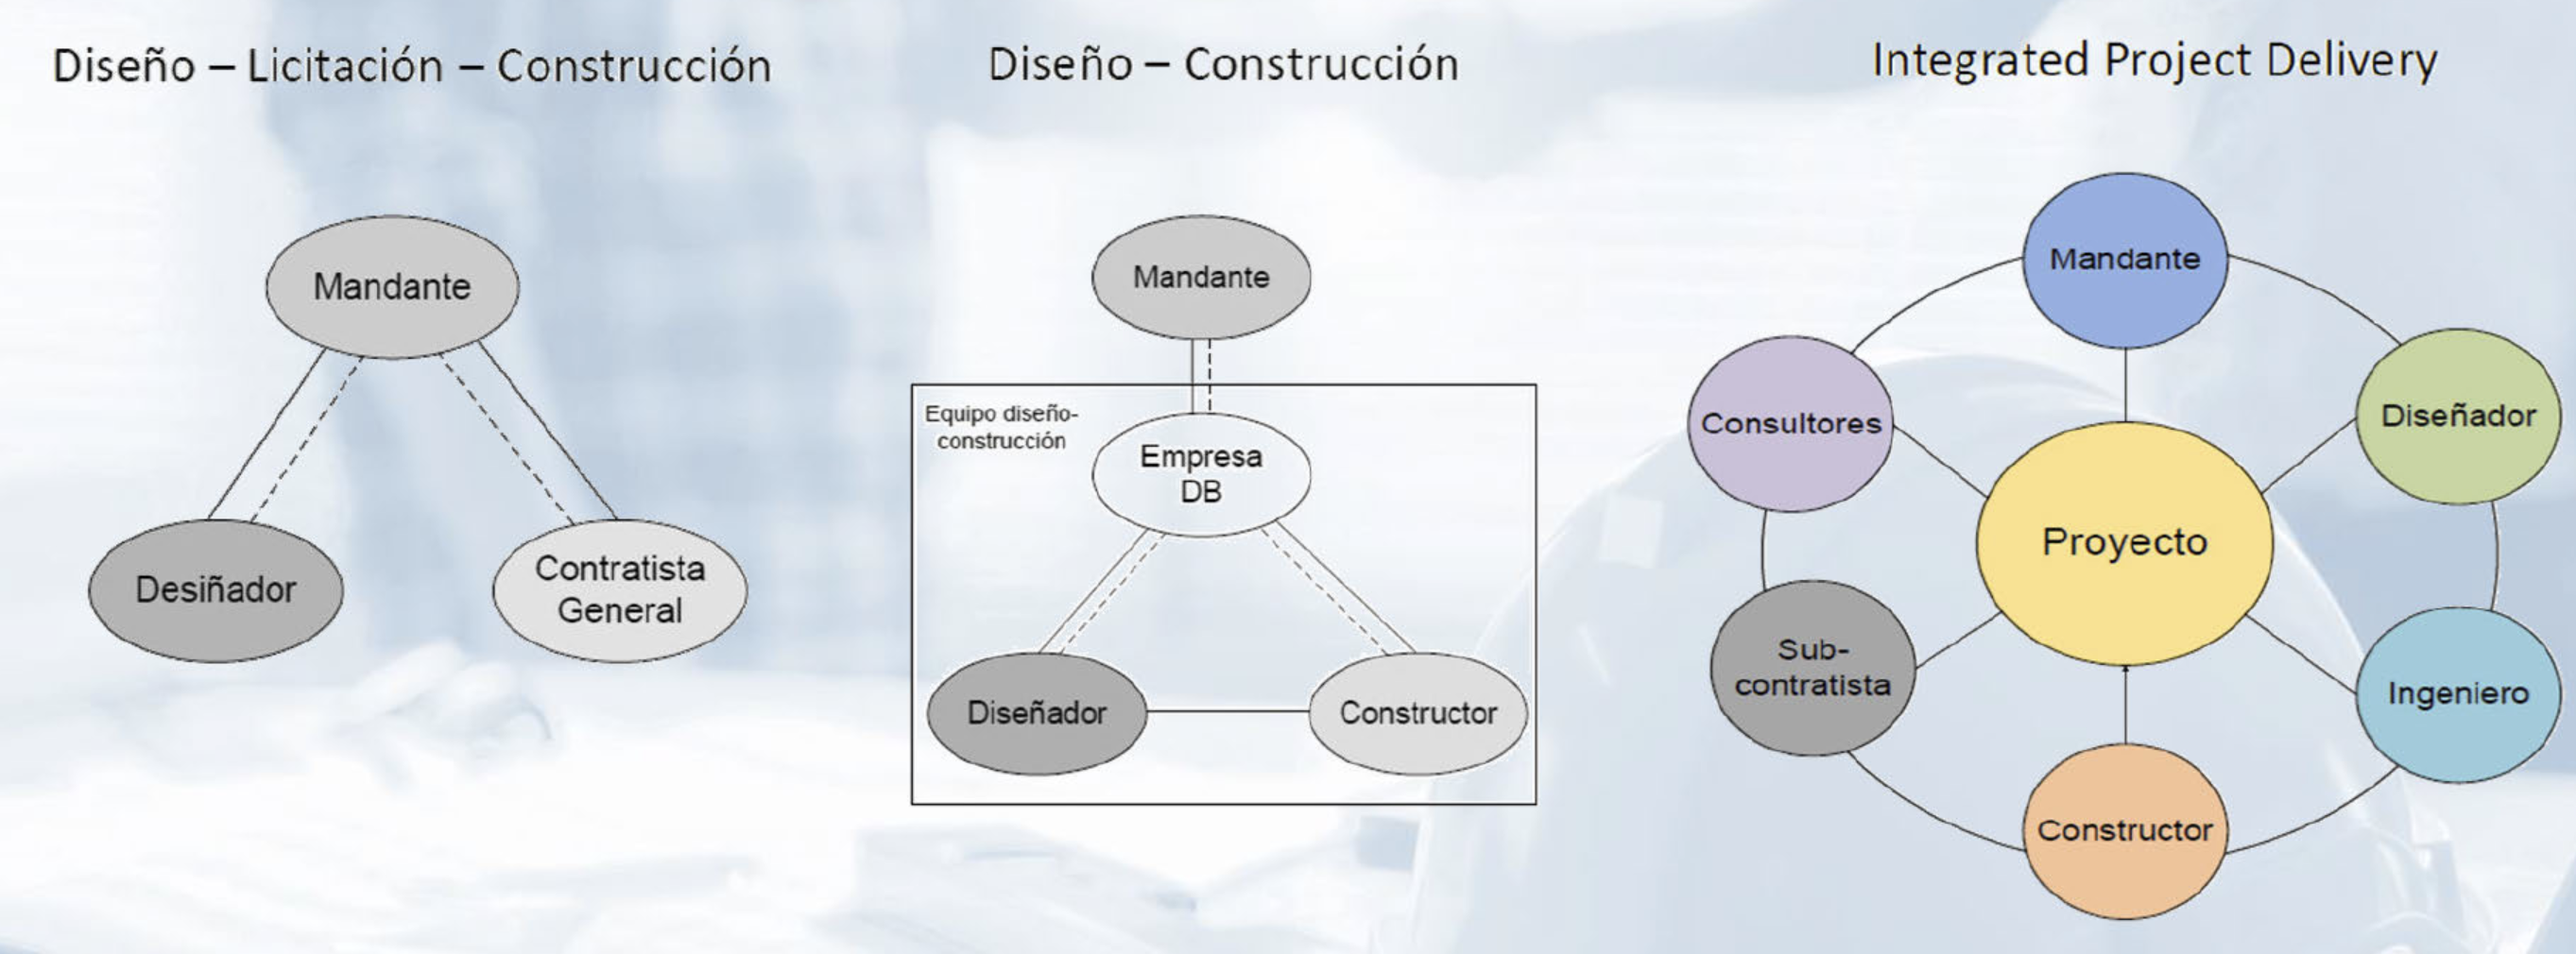
\includegraphics[width=0.8\textwidth]{IMAGENES/IPD.png}
\caption{Proceso de IPD}
\label{fig:ipd}
\end{figure}

De esta forma:

\begin{itemize}
    \item Se basa principalmente en la colaboración y la confianza.
    \item Genera buenos resultados siempre y cuando las personas se respeten mutuamente.
    \item Se centran en obtener buenos resultados para el proyecto y no se desvíen en lograr metas individuales.
\end{itemize}

Donde sus principios son:

\begin{itemize}
    \item Respeto mutuo y confianza
    \item Beneficio mutuo y recompensa
    \item Innovación colaborativa y toma de decisiones
    \item Definición temprana de objetivos
    \item Planificación intensificada
    \item Comunicación abierta
    \item Tecnología apropiada
    \item Organización y liderazgo
\end{itemize}

Y las etapas principales son:

\begin{itemize}
    \item Entrenamiento inicial: Metodología de gestión integrada de proyectos
    \item Validación y socialización de los principios y condiciones de satisfacción del proyecto
    \item Estructuración y definición de roles y responsabilidad del equipo participante, además del análisis y elección de metodologías y recursos a utilizar
    \item Aplicación de metodología y herramienta TVD
    \item Sustento legal que deberá ser definido y estructurado para llevar a cabo el proyecto, marcado por la colaboración y la innovación
\end{itemize}

Y los contratos relacionales son:

\begin{itemize}
    \item Ambiente de confianza, comunicación abierta y participación
    \item Cultura corporativa
    \item Trabajo colaborativo y reciprocidad
    \item Relaciones de largo plazo
\end{itemize}

\section{Metodologia Lean Construction}

\begin{figure}[H]
\centering
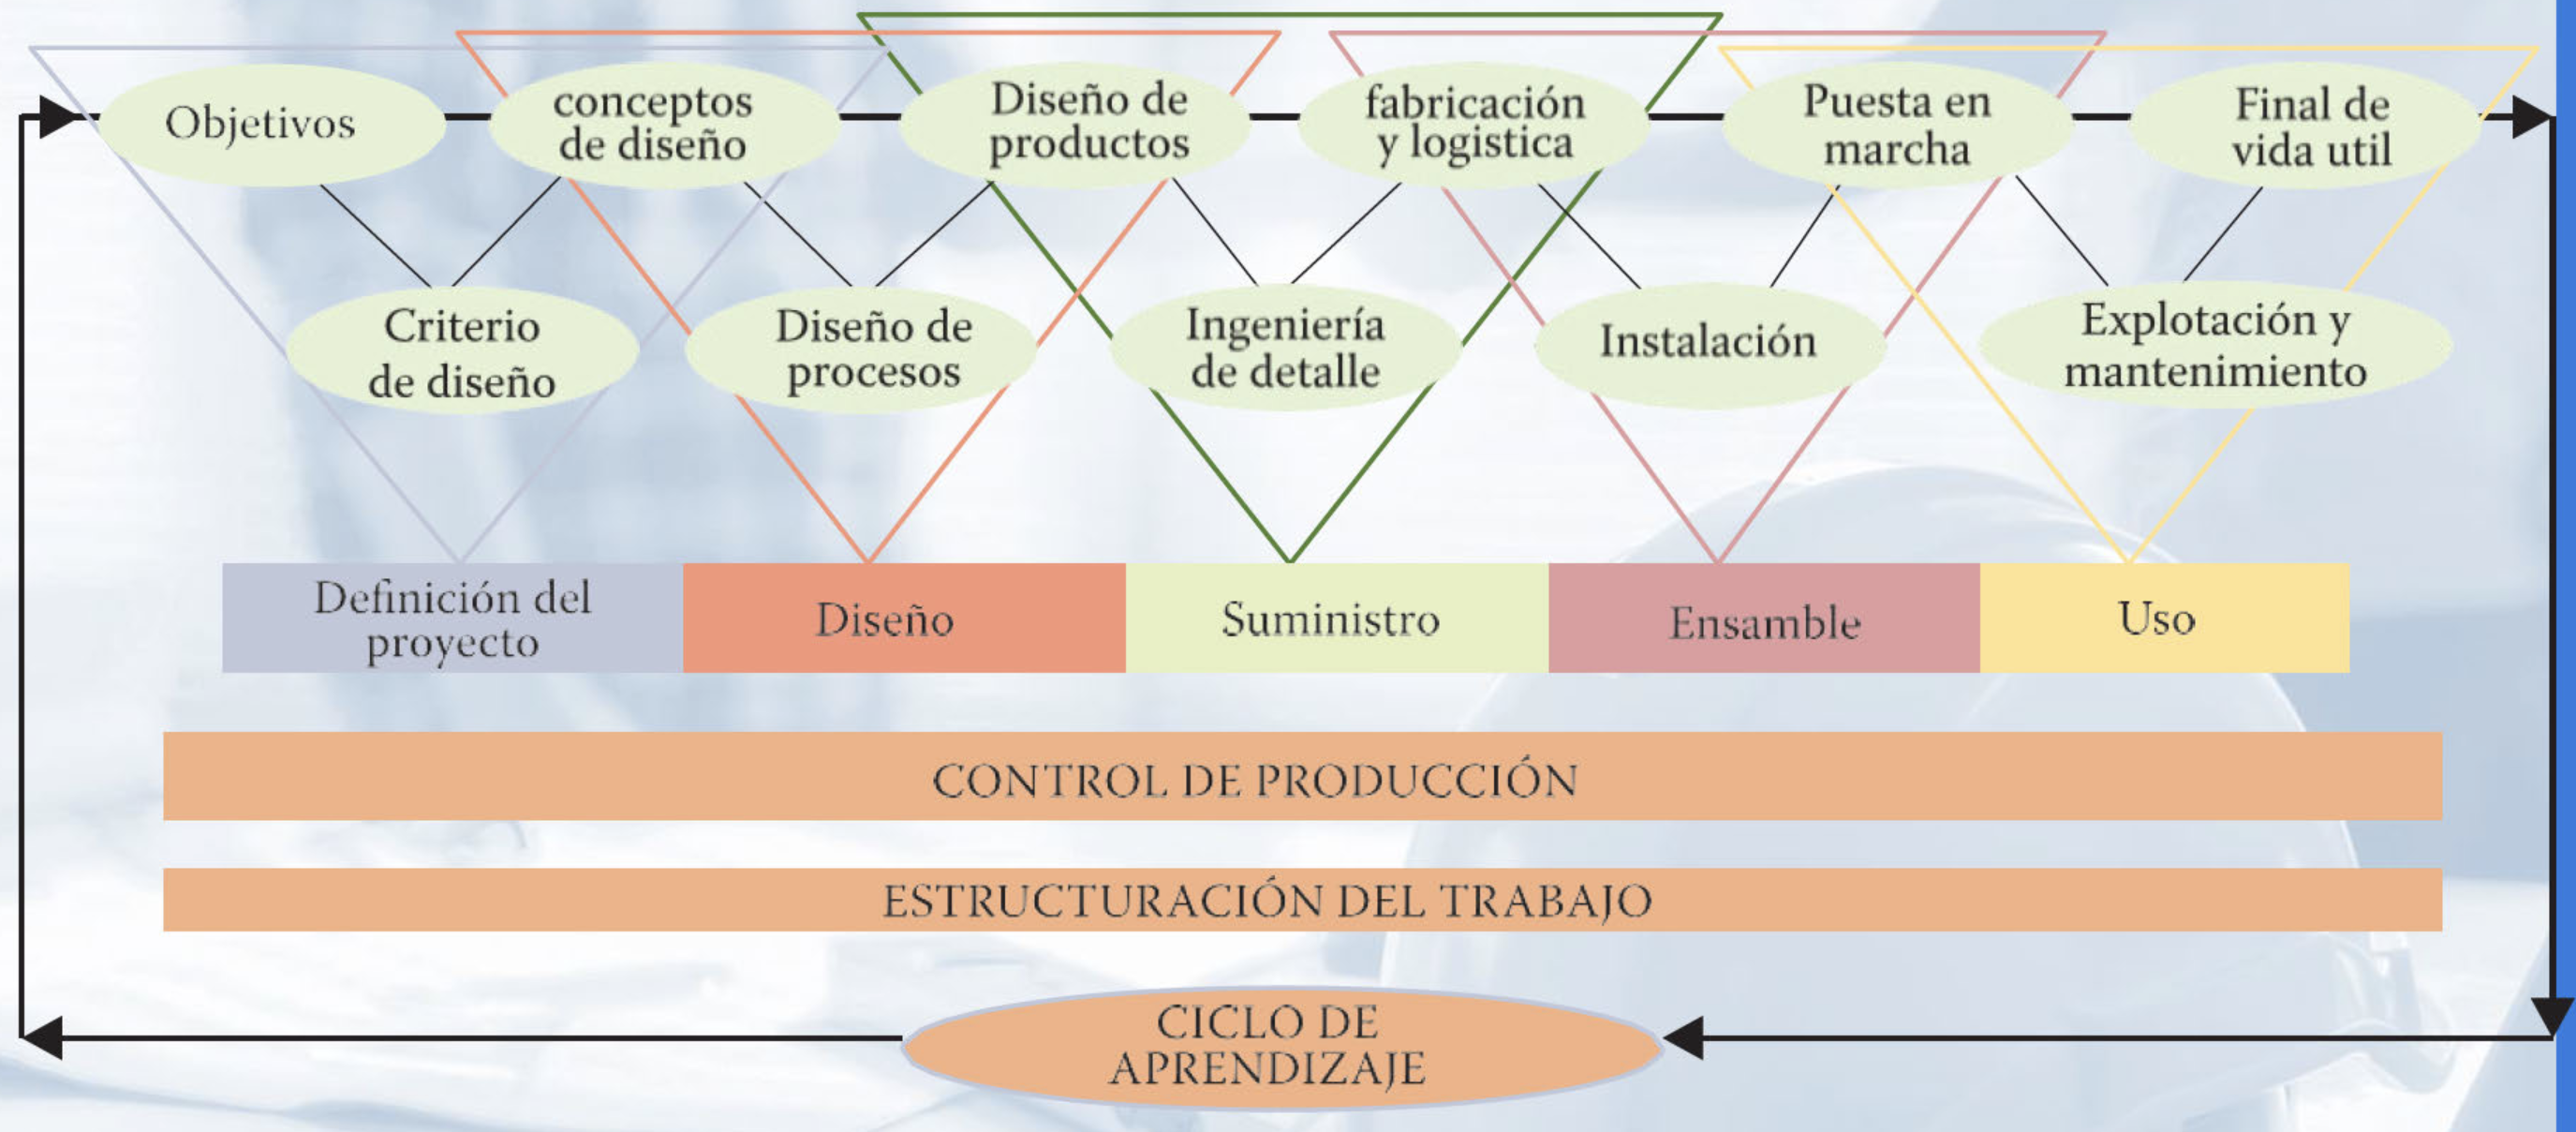
\includegraphics[width=0.9\textwidth]{IMAGENES/LEAN.png}
\caption{Proceso de Lean Construction}
\label{fig:lean}
\end{figure}



\section{Lean Construction}

\begin{itemize}
    \item Enfoque tradicional versus enfoque lean en la construcción.
    \item Modelos de flujo y de transformación.
    \item Principios del Lean Construction.
    \item Muda, Mura y Muri.
    \item Tipos de desperdicio en la construcción.
\end{itemize}

\subsection*{Comparación: Enfoque Tradicional vs Enfoque Lean en la Construcción}

\begin{table}[h]
    \centering
    \small
    \begin{tabular}{|p{6.5cm}|p{6.5cm}|}
        \hline
        \textbf{Enfoque Tradicional} & \textbf{Enfoque Lean} \\
        \hline
        Sigue modelo de transformación & Sigue el modelo de flujos \\
        \hline
        Primero se diseña el producto y después se diseñan los procesos & Los productos y procesos son diseñados conjuntamente \\
        \hline
        No todas las etapas del ciclo de vida del producto son consideradas durante el diseño & Todas las etapas del ciclo de vida del producto son consideradas durante el diseño \\
        \hline
        Las actividades se llevan a cabo tan pronto como sea posible & Las actividades se llevan a cabo al último momento responsable \\
        \hline
        Se eligen los subcontratistas en función del costo & Se eligen los subcontratistas debido a su capacidad de colaboración \\
        \hline
    \end{tabular}
    \caption{Comparación entre el enfoque tradicional y el enfoque Lean en la construcción}
\end{table}

\subsection*{Principios de Lean Construction}

\begin{enumerate}
    \item Reducción o eliminación de actividades que no agregan valor.
    \item Incremento del valor del producto considerando los requerimientos del cliente.
    \item Reducción de la variabilidad.
    \item Reducción del tiempo del ciclo.
    \item Simplificación de pasos, partes o enlaces.
    \item Incremento de la flexibilidad de la producción.
    \item Aumento de la transparencia del proceso.
    \item Enfoque del control al proceso completo.
    \item Mejoramiento continuo del proceso.
    \item Equilibrio entre el mejoramiento de flujos y el mejoramiento de la conversión.
    \item Benchmarking.
\end{enumerate}

\subsection*{Distribución del Trabajo}

\begin{itemize}
    \item \textbf{Trabajo Productivo (TP)}: Actividades que \textbf{agregan valor}.
    
    \item \textbf{Trabajo Contributorio (TC)}: Actividades que \textbf{sirven de apoyo y son necesarias}, pero \textbf{no agregan valor directamente}.
    
    \item \textbf{Trabajo No Contributorio o No Productivo (TNC)}: Actividades \textbf{innecesarias}, que tienen un \textbf{costo asociado} y \textbf{no agregan valor}.
\end{itemize}

\subsection*{Desperdicios}

\noindent Los \textbf{desperdicios} son cualquier elemento de producción, procesamiento o distribución que \textbf{no agrega valor} al producto final.

\vspace{0.3cm}

\noindent Los desperdicios \textbf{únicamente añaden costo y tiempo} a un proceso, sin contribuir al resultado esperado.

\subsection*{Desperdicios (Mudas)}

\begin{itemize}
    \item Transportación
    \item Defectos
    \item Sobreproducción
    \item Sobre-procesamiento
    \item Talento no utilizado
    \item Inventario
    \item Movimientos 
    \item Espera
\end{itemize}

\subsubsection*{Transportación}
Movimientos innecesarios de recursos (personas, equipos o materiales) desde un proceso a otro
Posibles causas:
\begin{itemize}
    \item Condiciones de terreno o proyecto
    \item Materiales no almacenados en la ubicación correcta
    \item Materiales recibidos con mucha anticipación
    \item Falta de plan logístico
\end{itemize}

\subsubsection*{Defectos}
Actividad que requiere retrabajo por errores u omisiones
Posibles causas:
\begin{itemize}
    \item Estándares de calidad mal definidos
    \item No seguir los procedimientos
    \item Falta de información
    \item Objetios no comunicados oportunamente   
\end{itemize}


\subsubsection*{Sobreproducción}
Ejecutar una actividad antes de que sea realmente necesarias
Posibles causas:
\begin{itemize}
    \item Falta de comunicación
    \item Adelantarse al Programa
    \item Deseo de ahorrar en mano de obra
    \item Deseo de moverse a otras actividades
\end{itemize}

\subsubsection*{Sobre-procesamiento}
Movimientos innecesarios en una obra de personas, equipos o materiales desde un proceso a otro. Esto puede incluir trabajo administrativo, así como actividades físicas.
Posibles causas:
\begin{itemize}
    \item Baja coordinación de equipos
    \item No conocer las especificaciones
    \item Contar con procesos poco optimizados
    \item Usar equipos excesivamente sofisticados
\end{itemize}

\subsubsection*{Esperas}
Interrupciones del trabajo o tiempo de inactividad o por falta de insumos
Posibles causas:
\begin{itemize}
    \item No saber qué es lo que se tiene que hacer
    \item Problemas no resueltos para un trabajo continuo
    \item Falta de equipamiento, herramientas o materiales
\end{itemize}

\subsubsection*{Movimientos}
Desplazamioentos innecesario de personal o maquinaria durante su trabajo, ya que dejan de producir durante su traslado
Posibles causas:
\begin{itemize}
    \item Falta de planificación
    \item Falta de organización
    \item No estudiar y aplicar los métodos más eficientes
    \item Problemas no resueltos para un trabajo continuo
\end{itemize}

\subsubsection*{Inventario}
Cantidad de materiales que va por sobre la necesidad inmediata. Además, de materiales puede incluir trabajo en proceso y productos terminados.
Posibles causas:
\begin{itemize}
    \item Problemas de planificación
    \item Poca confianza en los equipos de trabajo o equipo poco eficientes
    \item Falta de coordinación de equipos en obra
\end{itemize}


\subsubsection*{Talento no utilizado}
Desaprovechar el potencial de las personas en la organización
Posibles causas:
\begin{itemize}
    \item Falta de un método estándar para capturar ideas
    \item Cada nuevo proyecto es un nuevo inicio
    \item No incluir toda la cadena de producción en la planificación o soluciones
\end{itemize}

Bajando el nivel de desperdicios, exponemos los problemas reales: 
\begin{itemize}
    \item Tiempo excedente (buffers)
    \item dinero y materiales (inventario)
\end{itemize}

Meta:
\begin{itemize}
    \item Identificar Desperdicios
    \item Remover Desperdicios
    \item Revelar problemas
    \item Resolver los problemas
\end{itemize}

\textbf{Productos más rápidos, económicos y mejores}

\subsection{Cultura Lean}
\begin{itemize}
    \item Mejoramiento continuo.
    \item Respeto por las personas.
    \item Enfocarse en que todos piensen como empresa
    \item Competente
    \item Flexible
    \item Empoderados
    \item Motivados
\end{itemize}

Enfoque de arriba hacia abajo, donde pocos son recompensados $\rightarrow$ Ambiente de empoderamietno, con una fuerza laboral plenamente educada que disfrute de mayores incentivos

"Las personas no se resisten al Lean. Las personas se resisten a las formas en que perciben como Lean afectará sus vidas"

\begin{table}[h]
\centering
\begin{minipage}{0.45\textwidth}
\raggedright
\textbf{La gente resiste desafíos a su:}
\begin{itemize}
    \item Visión del mundo
    \item Narrativa
    \item Creencias
    \item Ego y autoimagen
\end{itemize}
\end{minipage}
\hfill
\begin{minipage}{0.45\textwidth}
\raggedright
\textbf{La gente ofrece resistencia por miedo a:}
\begin{itemize}
    \item Dolor al cambio
    \item Pérdida
    \item Seguridad
    \item Lo desconocido
\end{itemize}
\end{minipage}
\end{table}



\begin{table}[h]
\centering
\begin{minipage}{0.45\textwidth}
\raggedright
\textbf{Todos somos solucionadires de problemas:}
\begin{itemize}
    \item Aprende de los experimetos de otros
    \item Cuestionar los sesgos y supuestos
    \item Conoce sobre buenos argumentos y malos argumentos
    \item Planifica a largo plazo
    \item Define lo que debe y no se debe hacer
\end{itemize}
\end{minipage}
\hfill
\begin{minipage}{0.45\textwidth}
\raggedright
\textbf{Aprende de los experimentos de otros:}
\begin{itemize}
    \item El contexto y las condiciones son muy importantes
    \item No vayas directo a buscar respuestas o conclusioes de otros
    \item Resuelve tu problema específico
    \item Como un paciente responsable, no tomas medicina de otros
\end{itemize}
\end{minipage}
\end{table}


\newpage

\subsection*{Tecnología: Lean Construction}

\begin{multicols}{2}
    \begin{itemize}
        \item 5 porqués
        \item 6S
        \item 8 desperdicios
        \item Diagramas de causa y efecto
        \item DMAIC
        \item Flujo de valor
        \item Gemba
        \item Genchi genbutsu
        \item Gráficos de control
        \item Gráficos de Pareto
        \item Histograma
        \item Mapeo del flujo de valor (VSMA)
        \item Pensamiento y herramienta A3
        \item Planificar-hacer-estudiar-actuar (PDSA)
        \item Pull
        \item Trabajo equilibrado
        \item Trabajo estándar
        \item LPS
        \item VDC, TVD, entre otros
    \end{itemize}
\end{multicols}





\section{Administración de riesgos en un proyecto civil}

Existen tres categorías más importantes en la identificación de riesgos de proyectos IOC:
\begin{itemize}
    \item Riesgos de diseño
    \item Riesgos externos
    \item riesgos ambientales
    \item Riesgos organizacionales
    \item riesgos de administración de proyectos
    \item Riesgos legales y contractuales
    \item Riesgos de construcción
\end{itemize}

Estos riesgos se califican en función de su probabilidad de ocurrencia (del 1 al 5) y su impacto en el proyecto (del 1 al 5). La matriz de riesgos es una herramienta comúnmente utilizada para visualizar y priorizar estos riesgos.
A continuación, se presenta un ejemplo de una matriz de riesgos:
\begin{figure}[h]
    \centering
    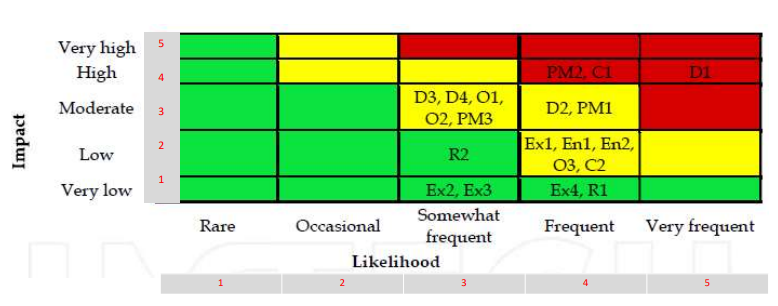
\includegraphics[width=0.8\textwidth]{Graficos/matriz.png}
    \caption{Matriz de riesgos de un proyecto IOC}
    \label{fig:matriz_riesgos}
\end{figure} 

Algunos ejemplos de riesgos que pueden surgir en un proyecto IOC son:
\begin{itemize}
    \item Riesgos de diseño: cambios en los requisitos del cliente, errores de diseño, falta de experiencia del equipo de diseño.
    \item Riesgos externos: cambios en la legislación, problemas con proveedores, condiciones climáticas adversas.
    \item Riesgos ambientales: contaminación del sitio, impacto en la fauna y flora local, problemas de salud pública.
    \item Riesgos organizacionales: falta de comunicación entre departamentos, conflictos internos, falta de recursos.
    \item Riesgos de administración de proyectos: falta de planificación adecuada, problemas con el cronograma, sobrecostos.
    \item Riesgos legales y contractuales: disputas contractuales, incumplimiento de normativas, problemas legales con terceros.
    \item Riesgos de construcción: accidentes laborales, problemas con subcontratistas, retrasos en la entrega de materiales.
\end{itemize}

También se puede hacer una matriz de evaluación de riesgos, que considera 7 factores:
\begin{itemize}
    \item Riesgo
    \item Repercusiones
    \item Probabilidad de que suceda
    \item Magnitud de las repercusiones
    \item Disparador de la acción 
    \item Responsable
    \item Plan de respuesta
\end{itemize}

Un ejemplo de matriz de evaluación de riesgos es el siguiente:
\begin{table}[h]
    \centering
    \small % Reduce tamaño de fuente
    \begin{tabularx}{\textwidth}{|c|X|c|c|X|c|X|}
        \hline
        \textbf{Riesgo} & \textbf{Repercusiones} & \textbf{Probabilidad} & \textbf{Magnitud} & \textbf{Disparador} & \textbf{Responsable} & \textbf{Plan de respuesta} \\
        \hline
        Clima adverso & + costos y retrasos & 3 & 4 & Pronóstico met. 2 días antes & Jefe de obra & Planificación de contingencias y ajustes al cronograma \\
        \hline
    \end{tabularx}
    \caption{Matriz de evaluación de riesgos}
\end{table}

Para poder calcular el riesgo se utiliza la siguiente fórmula:
\begin{equation}
    \text{Riesgo} = \text{Probabilidad} \times \text{Impacto}
\end{equation}
Si un riesgo tiene poca probabilidad y bajo impaccto, será capaz de aceparlo, pero si tiene alta probabilidad y alto impacto, se deberá prestar atención.

\section{Análisis de licitaciones, bases técnicas y contratos}

\subsection*{Etapa Inicial de un Proyecto OOCC}

\begin{itemize}
    \item Garantizar que el contratista/subcontratista comprenda los riesgos al hacer una oferta para un proyecto/servicio propuesto.
    \item El contratista/subcontratista puede incluir cantidades de reserva para contingencias en el precio de la oferta.
    \item El contratista/subcontratista puede desistir de presentar una oferta.
\end{itemize}

\subsection*{Criterios de Presentación de Presupuesto}

\begin{itemize}
    \item La oferta final se puede ver afectada por la estrategia que se haya tomado para la propuesta específica.
    \item El monto final puede bajar si el contratista tiene mucho interés en ganar el proyecto.
    \item El monto final puede subir si se tiene mucho trabajo en paralelo a este proyecto.
\end{itemize}

\subsection*{Decisión para Desarrollar una Propuesta}

\begin{itemize}
    \item La evaluación del contratista sobre la posibilidad de seguir o no con la preparación de una propuesta, en ocasiones se conoce como: \textbf{Decisión de Oferta / No Oferta}.
    \item Se pueden considerar los siguientes factores al decidir desarrollar una propuesta:
    \begin{itemize}
        \item Nuestras ventajas, fortalezas o capacidades diferenciadoras.
        \item Nuestras debilidades.
    \end{itemize}
\end{itemize}

\subsection*{Disminución / Mitigación de Riesgos}

\begin{itemize}
    \item Se pueden considerar los siguientes factores al decidir desarrollar una propuesta:
\end{itemize}

\begin{table}[h]
    \centering
    \small
    \begin{tabular}{|c|p{8cm}|c|p{4cm}|}
        \hline
        \textbf{N°} & \textbf{Factor} & \textbf{Puntuación (A/M/B)} & \textbf{Comentarios} \\
        \hline
        1 & Competencia & & \\
        \hline
        2 & Riesgo & & \\
        \hline
        3 & Consistencia con nuestra misión & & \\
        \hline
        4 & Oportunidad para ampliar nuestras capacidades & & \\
        \hline
        5 & Reputación con el cliente & & \\
        \hline
        6 & Disponibilidad de fondos & & \\
        \hline
        7 & Recursos disponibles para preparar propuesta de calidad & & \\
        \hline
        8 & Recursos disponibles para realizar el proyecto & & \\
        \hline
    \end{tabular}
    \caption{Planilla tipo de Lista de verificación de licitar/no licitar}
\end{table}

\noindent El \textbf{contratista} decidirá la acción de presentar su oferta:

\begin{center}
    \fbox{\textbf{Licitar \quad / \quad No Licitar}}
\end{center}

\subsection*{Factores que Influyen en la Decisión de Licitar / No Licitar}

\noindent Según un estudio, existen tres principales características de factores contribuyentes a la determinación final para licitar o no licitar en la industria de la construcción:

\begin{enumerate}
    \item Factores relacionados a la empresa,
    \item Factores relacionados al proyecto,
    \item Condiciones y expectativas del mercado, junto con consideraciones estratégicas.
\end{enumerate}

\noindent Estos factores pueden ser identificados:
\begin{itemize}
    \item Por el cliente, durante la etapa de elaboración de normativa o el llamado a propuesta (FRP) del proyecto.
    \item Por el contratista, durante la etapa de elaboración de su propuesta.
\end{itemize}

\noindent El \textbf{MANDANTE} decidirá acción de:
\begin{center}
    \fbox{\textbf{Adjudicar \quad / \quad No Adjudicar}}
\end{center}

\newpage
\section{Planificación y Gestión de Riesgos en Proyectos de Ingeniería Civil}

\subsection*{Evaluación de Riesgos}
Para manejar adecuadamente los riesgos en un proyecto, es necesario determinar:
\begin{itemize}
    \item La probabilidad de que ocurra cada riesgo.
    \item El impacto que tendría sobre los objetivos del proyecto.
\end{itemize}
Cada riesgo puede ser valorizado como alto, medio o bajo, o con valores numéricos(-1, 0, 1). Esto permite priorizar los riesgos según su probabilidad e impacto.

\subsection*{Plan de Respuesta ante Riesgos}
\begin{itemize}
    \item Se define un conjunto de acciones para evitar o reducir la probabilidad o el impacto de los riesgos.
    \item Cada riesgo debe tener un plan de acción y responsables asignados.
    \item Se utiliza una matriz de evaluación de riesgos como herramienta clave.
\end{itemize}

\subsection*{Implementación y Seguimiento}
\begin{itemize}
    \item Incluir reservas de contingencia en el presupuesto.
    \item Monitorear los riesgos identificados y detectar nuevos.
    \item Evaluar periódicamente la efectividad de las respuestas.
    \item Las reuniones de coordinación permiten actualizar los riesgos y documentar lecciones aprendidas.
\end{itemize}

\subsection*{Métodos de Identificación de Riesgos}
\begin{itemize}
    \item Lluvia de ideas con el equipo.
    \item Clasificación por categoría:
    \begin{itemize}
        \item Técnicos: nuevas tecnologías, estándares de calidad.
        \item Programación: retrasos de proveedores.
        \item Costo: variaciones por inflación o tiempo.
        \item Recursos Humanos: disponibilidad de personal.
        \item Externos: clima, regulación, stakeholders.
        \item Cliente: atrasos en pagos, aprobación de entregables.
    \end{itemize}
    \item Uso de experiencias aprendidas de proyectos anteriores.
\end{itemize}

\subsection*{Estimación de Impacto}
Por cada riesgo identificado se deben estimar los impactos potenciales:
\begin{itemize}
    \item Retrasos en el programa.
    \item Costos adicionales significativos.
    \item Riesgo de incumplimiento de especificaciones.
    \item Multas o penalizaciones contractuales.
\end{itemize}

\subsection*{Buenas Prácticas}
\begin{itemize}
    \item Asegurar una planificación detallada del alcance.
    \item Preparar paquetes de trabajo con anticipación.
    \item Revisar interferencias entre .
    \item Estimar correctamente la duración de actividades.
    \item Aplicar métodos como la ruta crítica (CPM).
    \item Hacer control y seguimiento continuo de los hitos.
\end{itemize}

\subsection*{Casos de Proyecto}
\begin{itemize}
    \item Instalación de torre grúa en obra.
    \item Diferencias de cubicación y su impacto económico.
    \item Generación y acumulación de residuos en faena.
\end{itemize}

\newpage
\section{Preguntas de Selección Múltiple y Respuestas Comentadas}

\subsection*{Pregunta 1}
\textbf{El material de video visto en clases Unidad 4, sobre análisis de riesgos dentro del sector construcción, analiza temas relacionados con:}
\begin{itemize}
    \item[A.] Criterios de Sustentabilidad en obras IOC
    \item[B.] Cambio de estrategia pública en obras de construcción
    \item[C.] \textbf{Riesgos compartidos en alza de precios de materiales entre cliente y contratista}
\end{itemize}

\textit{Comentario:} Esta fue la temática central del video de la Unidad 4, enfocado en cómo se abordan los riesgos financieros en contextos inflacionarios, destacando la importancia de compartir los riesgos contractuales.

\subsection*{Pregunta 2}
\textbf{¿A qué tipo de estudio de Evaluación Ambiental corresponde cuando el titular declara que el proyecto no generará ninguno de los efectos del Art. 11 de la Ley 19.300?}
\begin{itemize}
    \item[A.] \textbf{DIA (Declaración de Impacto Ambiental)} 
    \item[B.] EIA (Evaluación de Impacto Ambiental)
    \item[C.] Aplica realizar ambos estudios
\end{itemize}

\textit{Comentario:} La DIA es aplicable cuando se determina que el proyecto no produce efectos significativos. El EIA se requiere solo si alguno de los criterios del Art. 11 se ve afectado.

\subsection*{Pregunta 3}
\textbf{El método TVD (Target Value Design) contempla aplicar los siguientes criterios a la hora de abordar un proyecto de ingeniería:}
\begin{itemize}
    \item[A.] Todos los diseñadores se involucran desde el inicio
    \item[B.] El costo objetivo nunca debe ser excedido
    \item[C.] Compartir riesgos y recompensas
    \item[D.] \textbf{Todas las anteriores} 
\end{itemize}

\textit{Comentario:} Todos los ítems listados son principios fundamentales del TVD, el cual busca integración temprana, control de costos y colaboración entre actores del proyecto.

\subsection*{Pregunta 4}
\textbf{Dentro de Lean Construction, se indicó que uno de los desperdicios (mudas) que se presenta en tema de sobreproducción se refiere al exceso de materia prima, productos o procesos no en uso.}
\begin{itemize}
    \item[A.] \textbf{Verdadero}
    \item[B.] Falso
\end{itemize}

\textit{Comentario:} En Lean, la sobreproducción es uno de los ocho desperdicios. Generar más de lo necesario genera acumulación innecesaria, costos adicionales y uso ineficiente de recursos.

\section{Resolución de la Parte Teórica - Evaluación de Propuestas}

\subsection*{Cálculo de Nota Técnica}

La Oferta Técnica tiene una ponderación del 70\% y se compone de 5 criterios evaluados con un máximo de 80 puntos. Las ponderaciones específicas para cada criterio son:

\begin{center}
\begin{tabular}{|c|l|c|}
\hline
\textbf{Código} & \textbf{Criterio} & \textbf{Ponderación dentro de Nota Técnica (\%)} \\
\hline
X1 & Experiencia y antecedentes de la empresa & 25\% \\
X2 & Equipo de trabajo ofrecido               & 15\% \\
X3 & Seriedad de la oferta                    & 10\% \\
X4 & Capacidad económica                      & 20\% \\
X5 & Capacidad técnica                        & 30\% \\
\hline
\end{tabular}
\end{center}

Los puntajes por empresa son:

\begin{center}
\begin{tabular}{|c|c c c c c|}
\hline
\textbf{Empresa} & X1 & X2 & X3 & X4 & X5 \\
\hline
Empresa 1 & 55 & 35 & 70 & 20 & 80 \\
Empresa 2 & 45 & 65 & 65 & 50 & 70 \\
Empresa 3 & 35 & 45 & 55 & 45 & 55 \\
\hline
\end{tabular}
\end{center}

Aplicando las ponderaciones a cada empresa:

\begin{center}
\begin{tabular}{|c|c|}
\hline
\textbf{Empresa} & \textbf{Nota Técnica (70\%)} \\
\hline
Empresa 1 & $(55)(0.25) + (35)(0.15) + (70)(0.10) + (20)(0.20) + (80)(0.30) = 13.75 + 5.25 + 7.00 + 4.00 + 24.00 = \textbf{54.0}$ \\
Empresa 2 & $(45)(0.25) + (65)(0.15) + (65)(0.10) + (50)(0.20) + (70)(0.30) = 11.25 + 9.75 + 6.50 + 10.00 + 21.00 = \textbf{58.5}$ \\
Empresa 3 & $(35)(0.25) + (45)(0.15) + (55)(0.10) + (45)(0.20) + (55)(0.30) = 8.75 + 6.75 + 5.50 + 9.00 + 16.50 = \textbf{46.5}$ \\
\hline
\end{tabular}
\end{center}

\subsection*{Cálculo de Nota Económica}

Se asigna 80 puntos a la oferta más baja y se calcula el puntaje para las demás usando:

\[
\text{Puntaje empresa} = \left( \frac{\text{Oferta más baja}}{\text{Oferta empresa}} \right) \times 80
\]

\begin{itemize}
    \item Oferta más baja: Empresa 3 con 34.000 UF.
\end{itemize}

\begin{center}
\begin{tabular}{|c|c|c|}
\hline
\textbf{Empresa} & \textbf{Oferta Económica (UF)} & \textbf{Nota Económica (30\%)} \\
\hline
Empresa 1 & 35.500 & $\left(\frac{34000}{35500}\right) \times 80 = 76.5$ \\
Empresa 2 & 37.500 & $\left(\frac{34000}{37500}\right) \times 80 = 72.5$ \\
Empresa 3 & 34.000 & $80.0$ \\
\hline
\end{tabular}
\end{center}

\subsection*{Cálculo de Nota Final}

Se ponderan las notas técnica y económica:

\[
\text{Nota Final} = (\text{Nota Técnica}) \times 0.70 + (\text{Nota Económica}) \times 0.30
\]

\begin{center}
\begin{tabular}{|c|c|c|c|}
\hline
\textbf{Empresa} & \textbf{Nota Técnica (70\%)} & \textbf{Nota Económica (30\%)} & \textbf{Nota Final} \\
\hline
Empresa 1 & 54.0 & 76.5 & $(54)(0.70) + (76.5)(0.30) = 37.8 + 22.95 = \textbf{60.75}$ \\
Empresa 2 & 58.5 & 72.5 & $(58.5)(0.70) + (72.5)(0.30) = 40.95 + 21.75 = \textbf{62.7}$ \\
Empresa 3 & 46.5 & 80.0 & $(46.5)(0.70) + (80.0)(0.30) = 32.55 + 24.0 = \textbf{56.55}$ \\
\hline
\end{tabular}
\end{center}

\subsection*{Conclusión}

La propuesta se adjudica a la \textbf{Empresa 2}, ya que obtuvo la \textbf{mayor nota final} (62.7 puntos), producto de un buen equilibrio entre oferta técnica sólida y una oferta económica competitiva.


\section{Resolución Parte Teórica – Transferencia de Riesgos y Matriz de Evaluación}

\subsection*{2. Transferencia de Riesgos en Proyectos de Construcción}

Según el artículo \textit{"Risk Management in Construction Project"} revisado en clase, existen tres formas principales mediante las cuales un contratista puede transferir los riesgos en un proyecto de construcción:

\begin{enumerate}
    \item \textbf{Contratación de seguros:} 
    Utilizado para cubrir eventos fuera del control del contratista, como fenómenos climáticos extremos, robos, accidentes graves o fuerza mayor. Estos seguros permiten derivar la responsabilidad financiera a una aseguradora.

    \item \textbf{Subcontratación:}
    Delegar a terceros (subcontratistas) la ejecución de ciertas actividades específicas bajo condiciones definidas en contrato. Así, se transfieren riesgos como el cumplimiento de estándares de calidad, costos de materiales y cronogramas de ejecución.

    \item \textbf{Modificación de cláusulas contractuales:}
    Se establecen condiciones contractuales explícitas que distribuyen responsabilidades ante eventos específicos. Por ejemplo, en caso de alza de precios de materiales o trámites administrativos, se pueden definir cláusulas de riesgo compartido entre mandante y contratista.
\end{enumerate}

\vspace{0.3cm}

\subsection*{3. Análisis de Riesgos – Caso Rehabilitación de Pavimentos en Aeropuerto}

\textbf{Contexto:} \\
El proyecto consiste en la rehabilitación de losas de hormigón en la pista de aterrizaje del Aeropuerto Internacional Arturo Merino Benítez, en la Región Metropolitana. Este tipo de obras se realiza en zonas de alta criticidad operacional, bajo restricciones horarias estrictas, y con exigencias de calidad y precisión. Por lo tanto, gestionar adecuadamente los riesgos técnicos, logísticos y ambientales es esencial para el éxito del proyecto.

\vspace{0.3cm}

\subsubsection*{Riesgos Identificados y Cuantificación}

\begin{center}
\begin{tabular}{|c|p{8.2cm}|c|c|}
\hline
\textbf{ID} & \textbf{Riesgo} & \textbf{Probabilidad (1–5)} & \textbf{Impacto (1–5)} \\
\hline
A & Demora en el transporte de hormigón premezclado & 2 & 4 \\
B & Resistencia f’c del hormigón menor a la especificada en ensayo & 2 & 5 \\
C & Fisuras en las losas recién hormigonadas & 3 & 4 \\
D & Altas temperaturas durante ejecución y curado & 3 & 3 \\
E & Error en cubicación del volumen necesario de hormigón & 4 & 3 \\
F & Restricción horaria impide terminar colada a tiempo & 2 & 4 \\
G & Fallas en coordinación con torre de control / interrupciones operativas & 3 & 5 \\
H & Mal funcionamiento de maquinaria de colocación o vibrado & 2 & 4 \\
I & Ausencia o falla de moldajes en faena & 2 & 3 \\
\hline
\end{tabular}
\end{center}

\vspace{0.3cm}

\subsubsection*{Priorización de Riesgos}

Se consideran de prioridad alta los riesgos con mayor producto entre impacto y probabilidad.

\begin{center}
\begin{tabular}{|c|c|}
\hline
\textbf{Riesgos de Prioridad Alta} & B, C, G \\
\textbf{Riesgos de Prioridad Media-Alta} & A, D, E, F, H \\
\textbf{Riesgos de Prioridad Media o Baja} & I \\
\hline
\end{tabular}
\end{center}

\vspace{0.3cm}

\subsubsection*{Matriz de Evaluación de Riesgos (Ampliada)}

\begin{table}[H]
\centering
\resizebox{\textwidth}{!}{
\begin{tabular}{|c|p{5cm}|c|c|p{3cm}|p{2.5cm}|p{4cm}|}
\hline
\textbf{ID} & \textbf{Repercusiones} & \textbf{Prob.} & \textbf{Impacto} & \textbf{Disparador} & \textbf{Responsable} & \textbf{Plan de Respuesta} \\
\hline
A & Rechazo del hormigón o pérdida de trabajabilidad & 2 & 4 & Congestión en ruta de acceso & Jefe de Producción & Cambiar horario o ruta; prever camiones extra \\
\hline
B & Demolición y recarpetado por no alcanzar f’c & 2 & 5 & Ensayo a 3 días con baja resistencia & Jefe de Calidad & Aditivos acelerantes, uso de sensores para control temprano \\
\hline
C & Retrabajo por aparición de grietas post-curado & 3 & 4 & Inspección visual diaria & Supervisor de ejecución & Control estricto de curado y temperatura \\
\hline
D & Hormigón pierde trabajabilidad, fisuras por retracción & 3 & 3 & Temperatura ambiente sobre 30°C & Laboratorio & Añadir aditivos plastificantes y protección de losas \\
\hline
E & Sobras o déficit de hormigón, costos adicionales & 4 & 3 & Diferencia entre cubicación y pedido & Topógrafo/Jefe Obra & Revisar cubicación antes de cada jornada \\
\hline
F & Incompletitud de jornada por restricción horaria & 2 & 4 & Toque de queda operacional & Jefe de Producción & Reprogramar por bloques de faena + cuadrilla adicional \\
\hline
G & Paralización de obra por conflictos con tráfico aéreo & 3 & 5 & Cambio de prioridad operacional & Coordinador general & Planificar con torre de control; establecer ventanas horarias \\
\hline
H & Parálisis parcial por falla en equipos clave & 2 & 4 & Falla de equipo vibrador o mixer & Encargado de maquinaria & Mantención preventiva; backup de equipos críticos \\
\hline
I & Retardo de inicio por falta de moldajes & 2 & 3 & Revisión de check-list incompleto & Jefe de montaje & Revisar disponibilidad días antes, almacenamiento en obra \\
\hline
\end{tabular}
}
\caption{Matriz de evaluación de riesgos para rehabilitación de pavimentos en aeropuerto}
\end{table}



\end{document}
